\section{Aufgabe 11}
\subsection{a) }
    Zunächst galt es, mithilfe der Transformationsmethode Zufallszahlen
    entsprechend des Neutrinoflusses zu simulieren. Dieser ist gegeben
    durch
    \begin{equation*}
        \phi = \phi_0 \left( \frac{E}{\text{TeV}}\right)^{- \gamma}
    \end{equation*}
    Mit dem spektralen Index $\gamma = 2.7$ und der Normierungskonstante 
    $\phi_0$. Sie wird wie in Abbildung \ref{fig:norm} berechnet.

    \begin{figure}
        \centering
        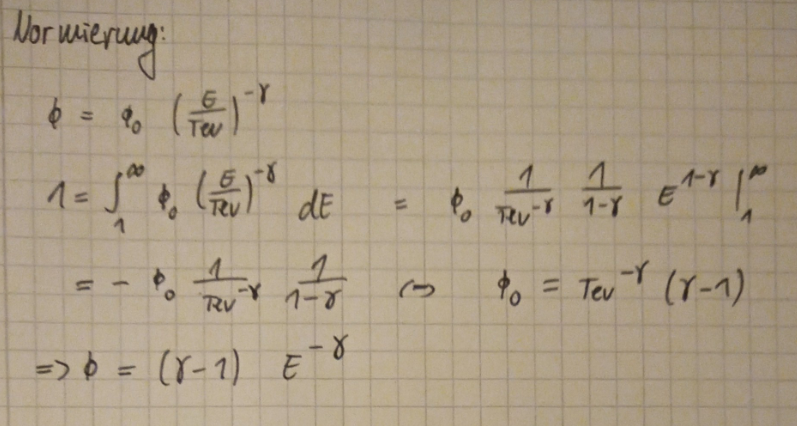
\includegraphics[width=\textwidth]{norm.png}
        \caption{Normierung des Neutrinoflusses.}
        \label{fig:norm}
    \end{figure}
    \FloatBarrier

    \noindent Daraufhin muss die Funktion integriert und invertiert werden,
    wie in Abbildung \ref{fig:inv} gezeigt.

    \begin{figure}
        \centering
        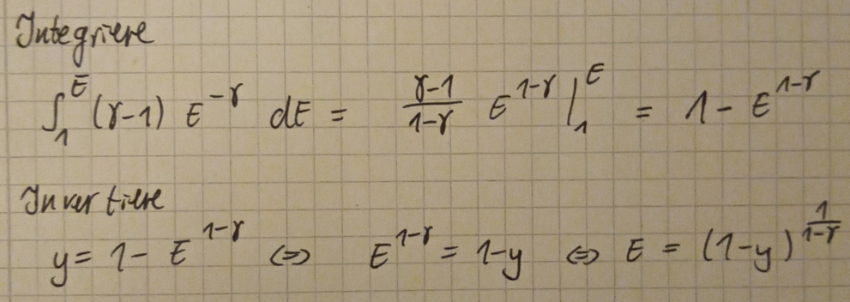
\includegraphics[width=\textwidth]{inv.png}
        \caption{Integration und Invertierung des Flusses.}
        \label{fig:inv}
    \end{figure}
    \FloatBarrier

    \noindent Mithilfe dieser Funktion werden nun gleichverteilte Zufallszahlen
    transformiert.

\subsection{b) Akzeptanz}
    Die Detektionswahrscheinlichkeit folgt der Verteilung
    \begin{equation*}
        P(E) = \left( 1 - e^{- \frac{E}{2}} \right)^3
    \end{equation*}
    Es wird das Neumann-Rückweisungsverfahren verwendet, um diese zu 
    berücksichtigen.

    \begin{figure}
        \centering
        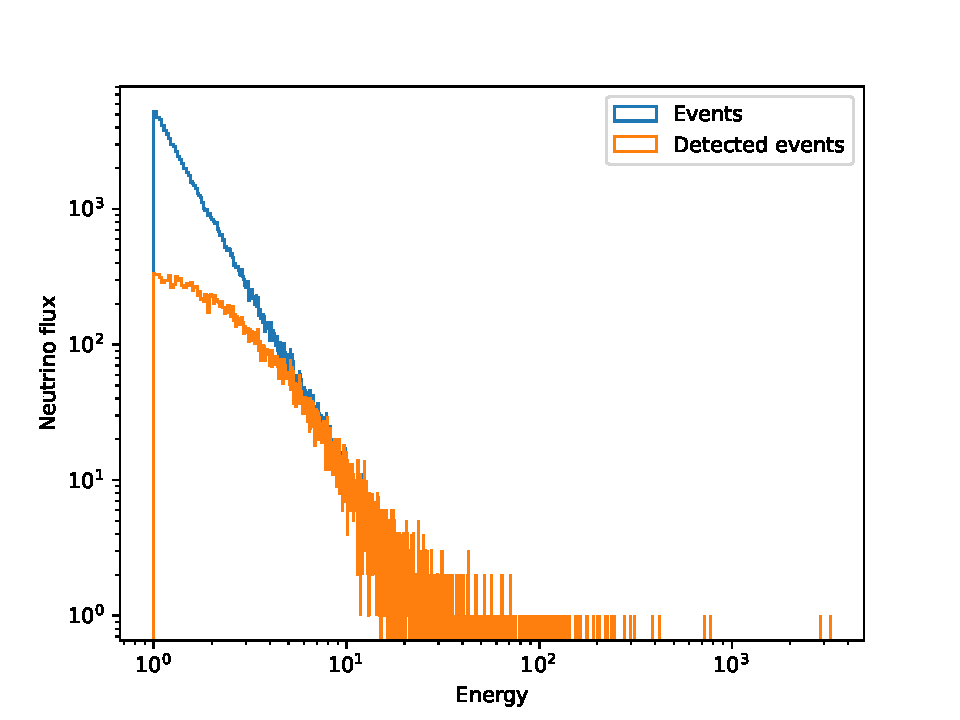
\includegraphics[width=\textwidth]{neutrinos.pdf}
        \caption{Events und Detektion.}
        \label{fig:det}
    \end{figure}
    \FloatBarrier

\subsection{c) Polarmethode}
    Gemäß der Vorlesung wird die Polarmethode implementiert. Die Ergebnisse der Tests sind in 
    Abbildung \ref{fig:polar} zu sehen.

    \begin{figure}
        \centering
        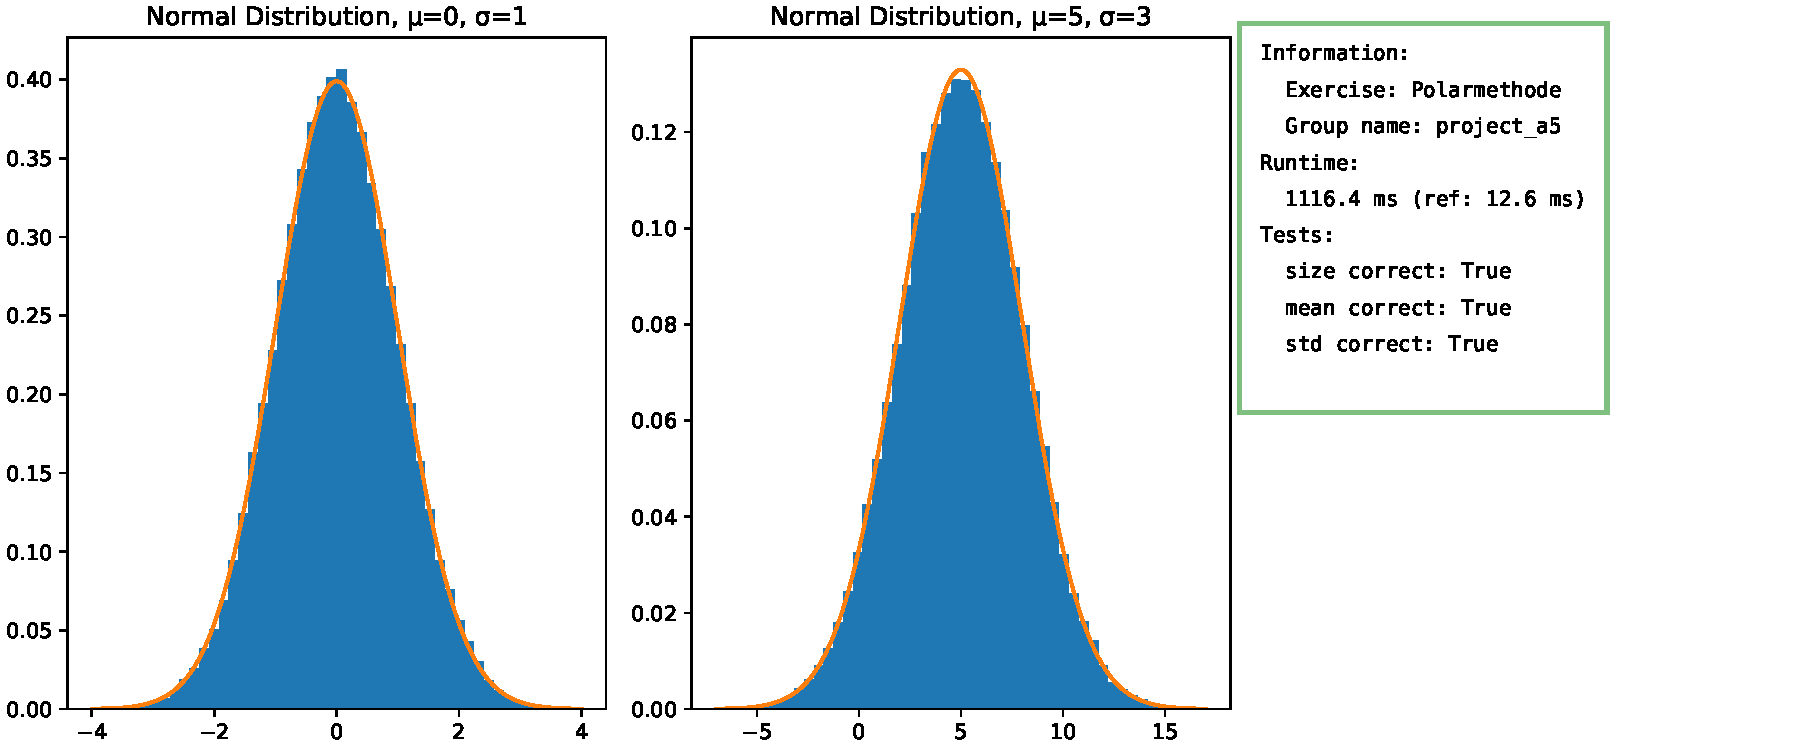
\includegraphics[width=\textwidth]{polar.pdf}
        \caption{Ergebnisse der Tests der Polarmethode.}
        \label{fig:polar}
    \end{figure}
    \FloatBarrier

\subsection{d) Energiemessung}
    Ein realer Detektor kann Ereignisse nicht absolut genau messen, stattdessen muss zum Beispiel die Zahl der Hits in Betracht gezogen werden.
    Dazu wird die für die Anzahl der Hits eine Normalverteilung mit Mittelwert $10 \cdot \frac{E}{\text{TeV}}$ und Standardabweichung $2 \cdot \frac{E}{\text{TeV}}$
    angenommen.\\

\subsection{e) Ortsmessung}
    Die Ortsauflösung ist ebenfalls energieabhängig, es gilt
    \begin{equation*}
        \sigma = \frac{1}{\text{log}_{10}(N + 1)}
    \end{equation*}
    Damit werden die x und y Koordinaten als normalverteilte Zufallszahlen zwischen 0 und 10 berechnet.

\subsection{f) Untergrund MC}
    Für den Untergrund werden $10^7$ Ereignisse simuliert, deren Zehnerlogarithmus einer Normalverteilung folgt. Diese ist in Abbildung \ref{fig:unter} dargestellt.\\
    Die Ortsvariablen hängen zusammen mit einem Korrelationskoeffizienten von $\rho = 0.5$. Dargestellt in einem zweidimensionalen Histogramm ergibt sich \ref{fig:unterort}.

    \begin{figure}
        \centering
        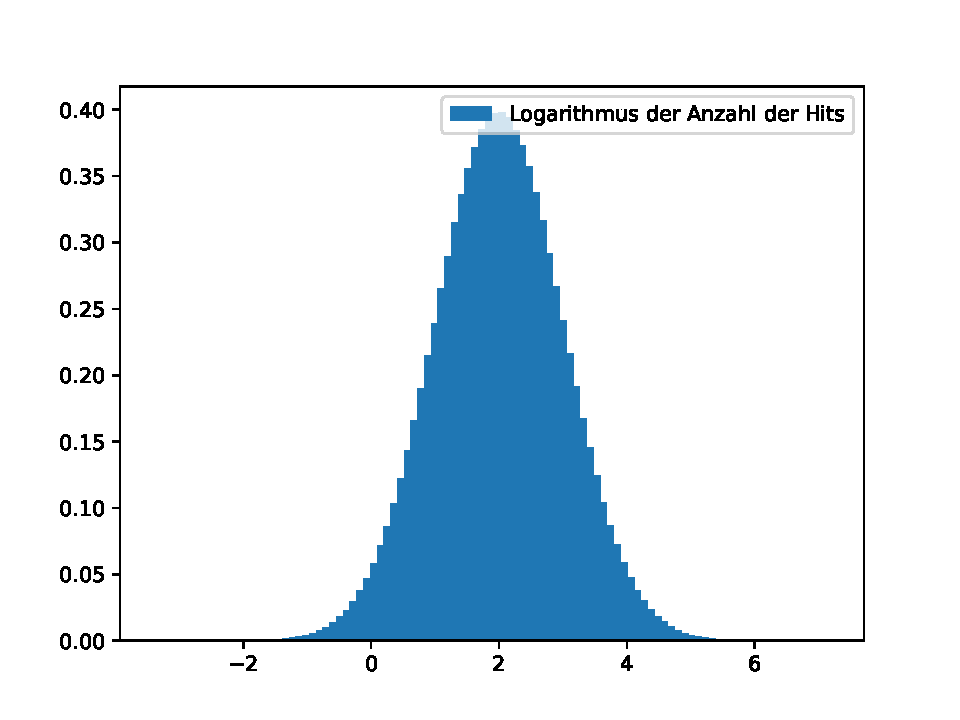
\includegraphics[width=\textwidth]{unter.pdf}
        \caption{Zehnerlogarithmus der Hits für den Untergrund.}
        \label{fig:unter}
    \end{figure}
    
    \begin{figure}
        \centering
        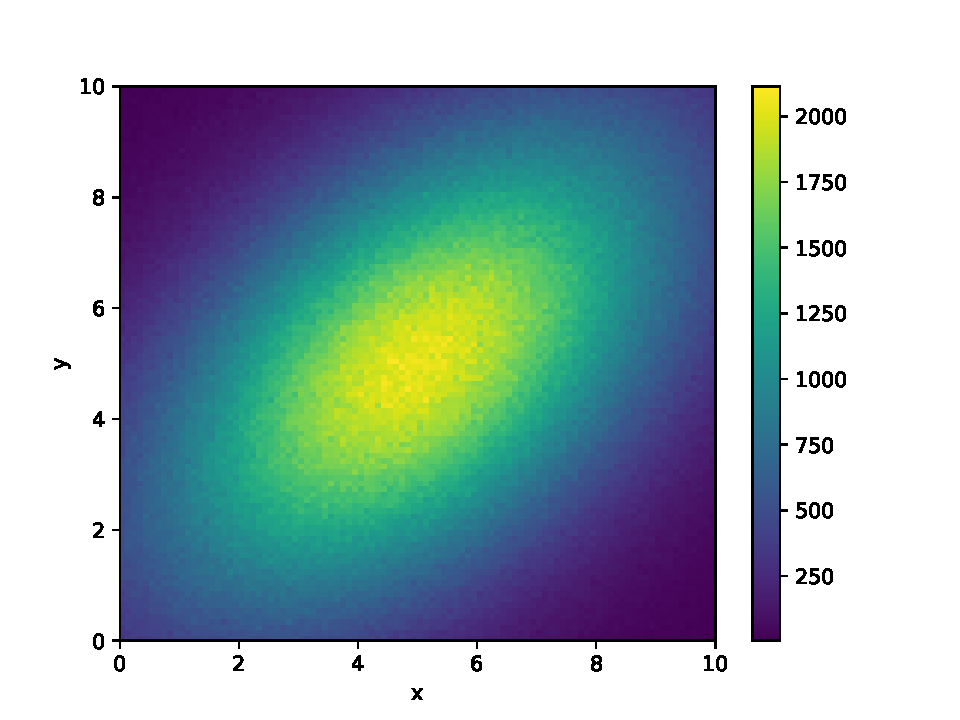
\includegraphics[width=\textwidth]{unterort.pdf}
        \caption{Ortsverteilung der Untergrund-Hits.}
        \label{fig:unterort}
    \end{figure}
    \FloatBarrier